% Guidance

To assist users who are less familiar with Cameo or MBSE, a full CubeSat Modeling How-To Guide has been included within the model. Users can double-click the document icon in Figure \ref{fig:Guidance} and open up a thorough guidebook that walks through each section and each diagram that users can fill out, in addition to guidance regarding the new Document Generator feature. The Guidance package also contains a set of modeling rules and a draft "active validation" profile to help identify common errors or missing data in the model. Figure \ref{fig:Modeling Rules} shows the structure of the included modeling rules, intended to keep the model standardized and to prevent common errors. Each of these rules is included in the Rules table with text descriptions. These are not mandatory to follow and these are only draft requirements created by the author. A wider conversation is required to establish modeling standards at AFIT, so these are just ideas to explore at a later date. 

\begin{figure}[H]
    \centering
    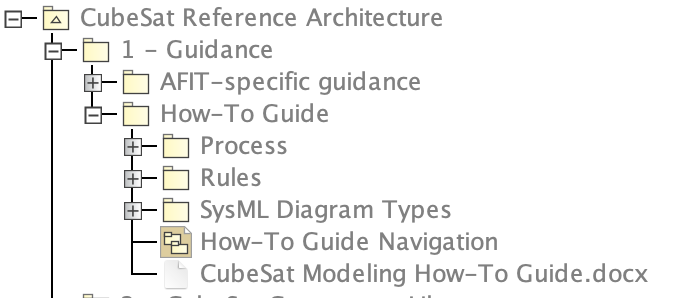
\includegraphics[width=4 in]{Thesis/Analysis_and_Results/Analysis and Results Figures/Guidance.png}
    \caption{Guidance}
    \label{fig:Guidance}
\end{figure}

\begin{figure}[H]
    \centering
    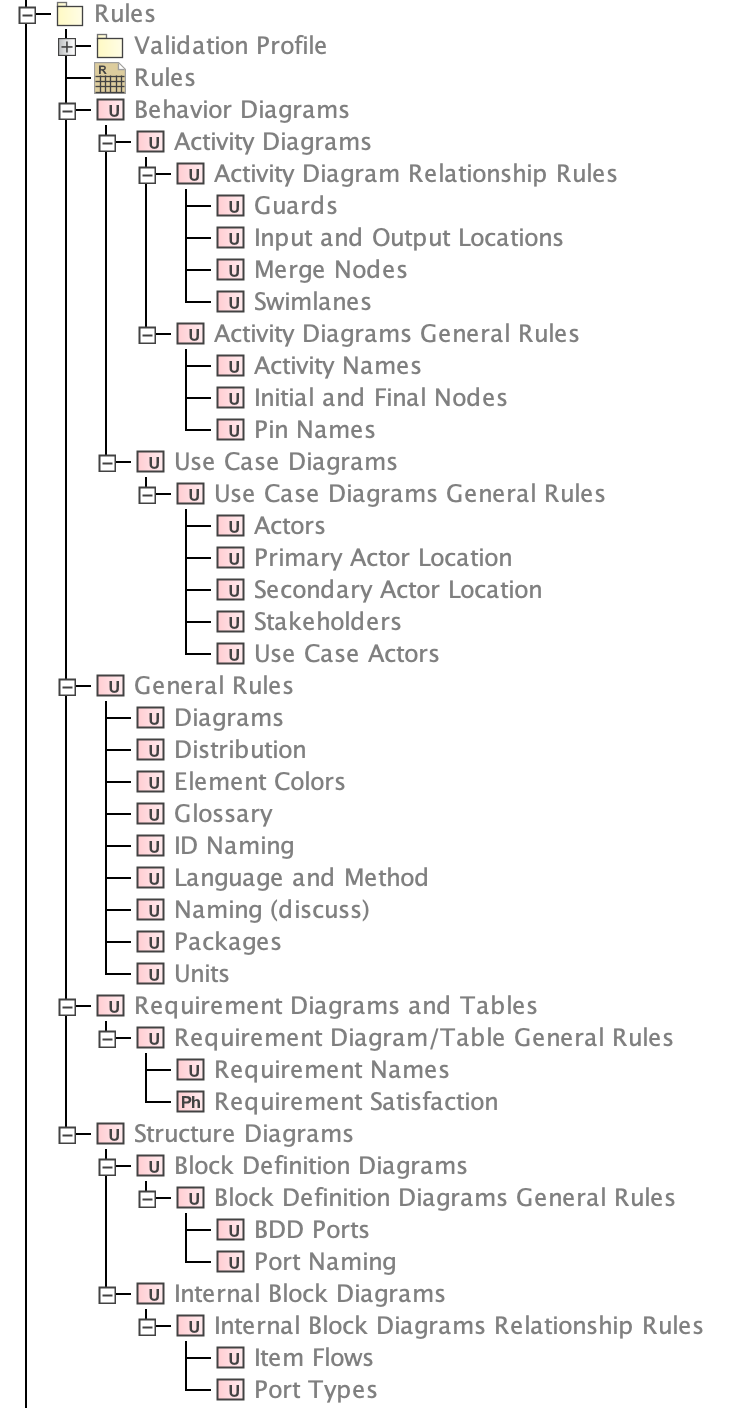
\includegraphics[width=3 in]{Thesis/Analysis_and_Results/Analysis and Results Figures/Rules.png}
    \caption{Modeling Rules}
    \label{fig:Modeling Rules}
\end{figure}

In addition to the modeling rules provided, a pared down version of SAIC's DE Validation Profile \citep{SAIC} is provided as well. As discussed in section \ref{Validation ruleset}, the Validation Profile does not meet the needs or practices of this model's intended audience, but there were several helpful active validation rules that were borrowed. A future effort may explore this concept further, but for now, roughly a third of the supplied rules were helpful for this context. Some very helpful rules include those that highlight when a requirement does not have proper traceability or is missing requirement text, rules that highlight missing elements in diagrams (such as starting and final nodes in activity diagrams), and a rule that checks to make sure each Value Property has an associated Value Type and Unit. If a modeler runs the validation profile during the design process, they may see helpful errors pointing out missing elements, so it does add some value to the Reference Architecture. 